%%%%%%%%%%%%%%%%%%%%%%%%%%%%%%%%%%%%%%%%%%%%%%%%%%%%%%%%%
\chapter[Results]{Results}
\label{chap:results}


\section{Most Informative Features} \label{sec:MostInformativeFeatures}

After training the Naive Bayes classifier with the manually categorized tweets and comments, the author
asked the classifier to show the 20 most informative features for it to recognize whether some text
should be classified positive, negative or neutral. Table 4.1 shows the results from the classifier.  \\

\begin{table}[h]
	\begin{center}
		\begin{tabular*}{10cm}{@{\extracolsep{\fill}} | r @{\hspace{1cm}} r @{\hspace{1cm}} l l r |  }
			\hline
			\multicolumn{5}{|c|}{Most Informative Features} \\
			\hline
			1 & starting = True & neu : pos & = & 21.5 : 1.0\\
			2 & great = True & pos : neg & = & 19.9 : 1.0\\
			3 & best = True & pos : neg & = & 12.8 : 1.0\\
			4 & world = True & pos : neg & = & 12.4 : 1.0\\
			5 & crossing = True & neu : pos & = & 7.2 : 1.0\\
			6 & thought = True & pos : neg & = & 7.1 : 1.0\\
			7 & player = True & neu : neg & = & 6.6 : 1.0\\
			8 & class = True & pos : neg & = & 6.4 : 1.0\\
			9 & shit = True & neg : pos & = & 6.2 : 1.0\\
			10 & good = True & pos : neg & = & 5.1 : 1.0\\
			11 & better = True & pos : neg & = & 4.9 : 1.0\\
			12 & fucking = True & neg : pos & = & 4.4 : 1.0\\
			13 & flicks = True & pos : neg & = & 3.4 : 1.0\\
			14 & decision = True & neg : pos & = & 3.3 : 1.0\\
			15 & even = True & neg : pos & = & 2.7 : 1.0\\
			16 & much = True & neg : pos & = & 2.7 : 1.0\\
			18 & can't = True & neg : pos & = & 2.7 : 1.0\\
			19 & like = True & pos : neg & = & 2.6 : 1.0\\
			20 & least = True & pos : neg & = & 2.6 : 1.0\\
			\hline
		\end{tabular*}
	\end{center}
	\caption{ Most informative features from the manually categorized tweets }
\end{table}

\newpage
\section{Results webpage} \label{sec:ResultsWebpage}

Below is a screenshot taken of the webpage created after running the program with the search parameters "MUFC Basel" which refer to the English team Manchester United Football Club and the Swiss football club Basel. \\

\begin{figure}[h]
	\centering
		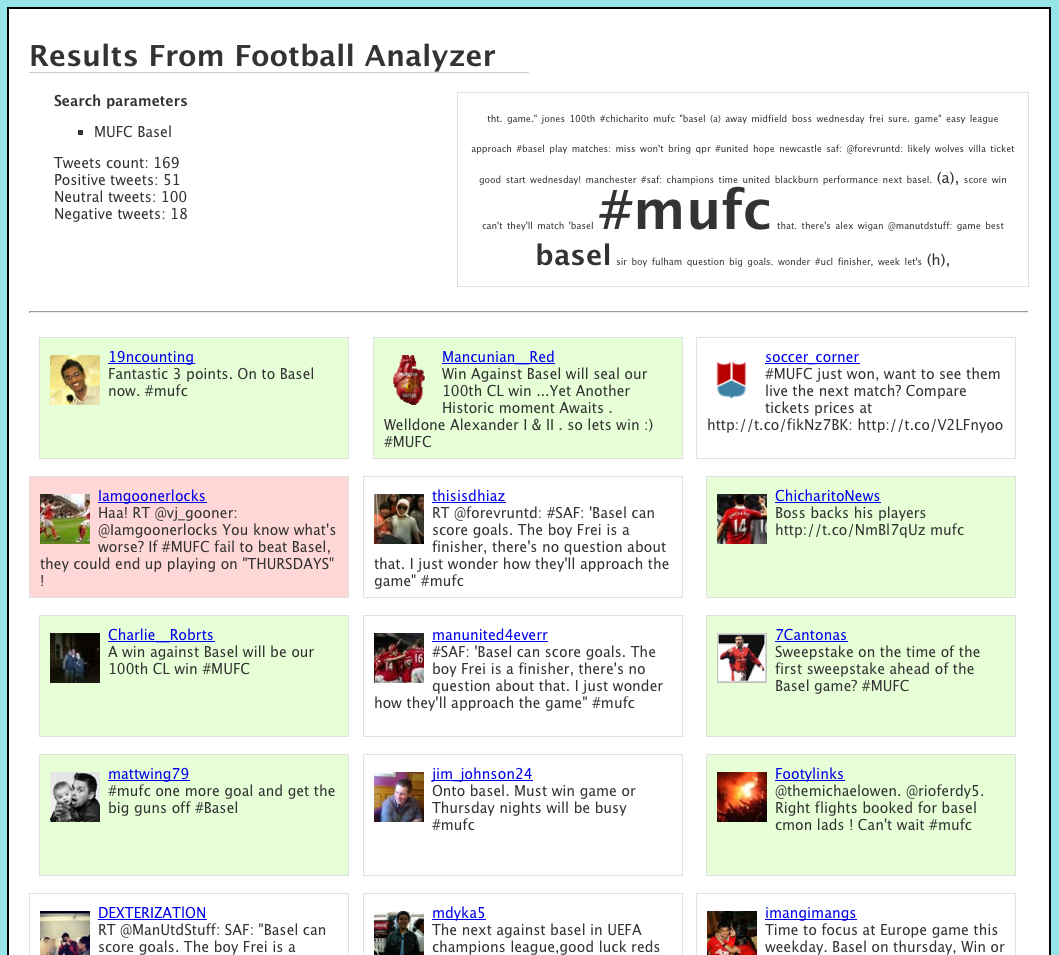
\includegraphics[width=400px]{images/webpage.png}
	\caption{ Screenshot of the results webpage }
	\label{fig:results}
\end{figure}

%To section \ref{sec:eqnom}
